\documentclass{article}
\usepackage[margin=1in]{geometry}
\usepackage{amsmath}
\usepackage{amsfonts}
\usepackage{amsthm}
\newtheorem{claim}{Claim}
\usepackage{algorithm}
\usepackage[noend]{algpseudocode}
\usepackage{mdframed}
\usepackage{mathtools}
\usepackage{tikz}
\usepackage{graphicx}
\usetikzlibrary{arrows}
\usepackage{subcaption}
\DeclarePairedDelimiter\ceil{\lceil}{\rceil}
\DeclarePairedDelimiter\floor{\lfloor}{\rfloor}
\title{CS 330: Homework 2}
\author{Michael Lin}
\begin{document}
\maketitle

\section*{Problem 1}
A graph is bipartite if the graph has no cycles or if all cycles have a even number of elements. We will use BFS search to determine if the cycles have even number of elements.
\begin{algorithm}
\caption{Determine if graph is bipartite}\label{prob1}
	\begin{algorithmic}[1]
	\Function{bfs}{node $s$, graph $G(V,E)$}
	\For {all $u\in V$} $d(u)=\infty$
	\EndFor	
	\For {all $s \in V$}
		\If{$s$ is unmarked}
			\State $d(s)=0$, mark $s$
			\State $Q = \emptyset$
			\State enqueue($s,Q$)
			\While{$Q \neq \emptyset$}
				\State $u=$dequeue$(Q)$
				\For {all $(u,v)\in E$}
					\If {$d(v)=\infty}$
						\State $d(v)=d(u)+1$, mark $v$
						\State enqueue($v, Q$)
					\Else
						\If {$d(v)-d(u)$ is even}
							\State \Return``graph is not bipartite"
						\EndIf
					\EndIf
				\EndFor
			\EndWhile
		\EndIf
	\EndFor
			\State \Return ``graph is bipartite"
	\EndFunction
	\end{algorithmic}

\end{algorithm}
\begin{proof}[Proof of correctness]
If the graph has no cycles, then starting from source $s$, every other node is in set $A$ and all other nodes are in set $B$, which implies bipartite. Similarly, in a cycle with even number of elements, choose any node to begin and place this node in set $A$. Following the path, the second node will be in set $B$, as well as every $n$th node where $n$ is even. Every other node is odd, and will be in set $A$. Thus, the graph is bipartite.

The algorithm uses BFS to search the entire graph, and will also detect a cycle when it returns to node $v$ and sees $d(v)\neq \infty$ since this means $v$ has already been visited. In this case, determining if $d(v)-d(u)$ is even is sufficient to say graph is not bipartite. To see this, suppose the index of the first element in the cycle is $i$. If number of elements in the cycle, say $k$, is odd, then the index of the last element is $i+k-1$, which is even if $i$ is even or odd if $i$ is odd. Thus the difference between the indices, which is $i+k-1-i=k-1$, which is even.
\end{proof}

\begin{proof}[Proof of runtime]
BFS has $O(|V|+|E|)$ runtime; the algorithm above only add constant work of computing $d(v)-d(u)$ to BFS. Thus the algorithm also has $O(|V|+|E|)$ runtime.
\end{proof}
\pagebreak

\section*{Problem 2}
To find an algorithm that determines whether there is a node from which all other nodes are reachable, first observe that the following claim is true:
\begin{claim}
If $s\in V$ is the only source in $G$, then all nodes are reachable from $s$.
\end{claim}
\begin{proof}
Prove by contrapositive. Suppose we are given a directed acyclic graph $G(V,E)$. By Dasgupta p. 97, $G$ has a source $s \in V$. Suppose there is a node $v\in V$ not reachable from $s$. If $v$ is a distinct component (i.e. not in the same component as $s$), then $v$ is also a source. If $v$ is in the same component as $s$, then $v$ can only be a predecessor of any node in $V$, which by definition means $v$ is a source. In either case, $s,v$ are both sources, which means there are more sources. Since the contrapositive is true, therefore the original claim is true.
\end{proof}
Given the above claim, we only need to find an algorithm that would check to see if $G$ has only one source. This is simple: first, we store all nodes as keys in a Hashmap with values set to 0. Then, we iterate through the adjacency list for every node. For every adjacent node we find in the adjacency list, update the value corresponding to that node in the Hashmap to 1. At the end, look at the number of 0's in all the values of the keys. If we only find one 0, then there is only one source in $G$.
\begin{proof}[Proof of correctness]
The algorithm looks at the nodes in each adjacency list and essentially determines which nodes are not successors. The counting the number of such nodes would tell us if there is only one such node.
\end{proof}
\begin{proof}[Proof of runtime]
Since we iterate through every node, we first have $O(|V|)$. At the same time, going through every adjacency list looks at every edge, which means another $O(|E|)$. Recall that insertion and search operations on Hashmap are both $O(1)$. Creating the Hashmap, therefore, takes $O(|V|)$ time. Since we check and update the values in the Hashmap for every edge, thus this makes $O(|E|)$ time. Determining number of 0's in al the values of the keys takes $O(|V|)$ time. Altogether, we have $O(3|V| + 2|E|)$, which is $O(|V|+|E|)$.
\end{proof}
\pagebreak

\section*{Problem 3}
\begin{algorithm}
\caption{Finding shortest cycle}
\begin{algorithmic}[1]
\Function{Cycle}{graph $G(V,E)$}
\For{all $s\in V$}
	\State \textsc{Dijkstra}$(s,G)$ \Comment{Output from \textsc{Dijkstra} is $d(s,u)$, for all $u\in \{V-s\}$; $\infty$ if unreachable.}
\EndFor
\State Find the set $D = \{d(s,u)+d(u,s)|s,u\in V\}$
\State Add 0 to $D$
\State \Return Minimum value in $D$
\EndFunction

\end{algorithmic}
\end{algorithm}

\begin{proof}[Proof of correctness]
\textsc{Dijkstra} ensures that we find the shortest path between any two nodes in a graph. Suppose $u,v \in G$. Consider 2 cases:
\begin{enumerate}
	\item Suppose $u$ can reach $v$, and $v$ can reach $u$. This means $u$ and $v$ are part of a cycle. Because \textsc{Dijkstra} gives shortest paths $d(u,v)$ and $d(v,u)$, their sum will be the length of the shortest cycle involving $u$ and $v$. If this sum is the smallest element in the set $D$, then the algorithm will correctly return it as the length of the shortest cycle.
	
	\item Suppose at least one of the nodes cannot reach the other one. Without loss of generality, suppose $u$ can reach $v$, but $v$ cannot reach $u$. This means $u$ and $v$ are not part of the same cycle, and $d(v,u)=\infty$. Thus, the sum of $d(u,v)$ and $d(v,u)$ will also be $\infty$ (this would still be true if neither node could reach the other since $d(u,v)$ would also be $\infty$). Because we add 0 to the set $D$, the sum $d(u,v)+d(v,u)$ will never be returned, which is correct.
\end{enumerate}
Because all elements in $D$ are nonnegative, the algorithm will correctly return 0 if there are no cycles, and will correctly return the shortest cycle otherwise.
\end{proof}

\begin{proof}[Proof of runtime]
Implement priority queue in \textsc{Dijkstra} with array gives a runtime of $O(|V|^2)$ (see Dasgupta p. 119). Iterating through every node thus takes $O(|V|^3)$. Finding $D$ looks at every edge once; since there are at most $|V|^2$ edges, this part takes $O(|V|^3)$, thus doesn't add to the overall runtime. Similarly, adding 0 to $D$ and finding the minimum value in $D$ all take less than $O(|V|^3)$. Therefore, the overall runtime is $O(|V|^3)$.
\end{proof}

\pagebreak

\section*{Problem 4}
\begin{algorithm}
\caption{Finding nodes with unique shortest path}
\begin{algorithmic}[1]
\Function{Unique}{node $s$, graph $G(V,E)$}
\For {all $u\in V$}
	\State $d(u)=\infty$, $h(u)=\infty$
\EndFor
\State $d(s)=0$, $h(s)=0$, $Q=\emptyset$
\State \textsc{insert}($s,Q$)
\While {$Q\neq \emptyset$}
	\State $u = \textsc{ExtractMin}(Q)$
	\For{all $(u,v)\in E$}
		\If {$d(v)>d(u)+c(u,v)$} $d(v)=d(u)+c(u,v)$
		\ElsIf {$d(v)=d(u)+c(u,v)$} $h(v)=d(v)$
		\EndIf
		\State \textsc{DecreaseKey}$(v)$
	\EndFor
\EndWhile
\For{all $u\in V$}
	\If{$d(u)=h(u)$} \textsc{mark}($u$)
	\EndIf
\EndFor
\State \Return all unmarked nodes
\EndFunction
\end{algorithmic}

\end{algorithm}

\begin{proof}[Proof of correctness]
The algorithm uses \textsc{Dijkstra}, which ensures shortest path from $s$. From here, we added another distance variable $h(v)$ for all $v\in V$, which is updated only if we had already found at least another path from $s$ to $v$ with same distance as the currently tested path. Thus, $d(v)\leq h(v)$ is always true, and the equality is true only when the shortest path is not unique. The final for loop in the algorithm marks all nodes that do not have unique shortest path from $s$, which includes $s$ itself since in Line 4, we set $d(s)=h(s)=0$. If a node $u$ cannot be reached, then $d(u)=h(u)=\infty$, which will also be marked. All other unmarked nodes either only have one path (thus shortest path) from $s$, in which case $d(\cdot)<\infty$ and $h(\cdot)=\infty$, or have a unique shortest path, in which case $d(\cdot)<h(\cdot)<\infty$. Returning these unmarked nodes gives the correct answer.
\end{proof}

\begin{proof}[Proof of runtime]
Lines 1-11 are identical to \text{Dijkstra} plus additional constant time operations, which, from lecture, has $O( (|V|+|E|)\log |V|)$ runtime if implementing priority queue with binary heaps. The final for loop, which iterates through every node once, takes $O(|V|)$ time, which does not add to the overall runtime. Thus, this algorithm runs in $O( (|V|+|E|)\log |V|)$.
\end{proof}


\pagebreak

\section*{Problem 5}


\begin{itemize}
\item {\bf Does the minimum spanning tree change?} No. Suppose we always use same algorithm to find minimum spanning tree. Consider Kruskal's algorithm, which we know from lecture is correct. The minimum spanning tree is directly dependent on the sorting order of the weights. Adding 1 to the weight of each edge does not change the sorting order. Thus, the minimum spanning tree would not change.
\item {\bf Do the shortest paths change? } Yes. In the graph with original weights, the shortest path from A to D is through B and C ($1+1+1=3<4$). However, adding 1 to the weight of each edge makes the shortest path from A to D as the direct path ($2+2+2=6>5$).

\begin{figure}[h]
\centering
\begin{subfigure}[h]{0.3\textwidth}
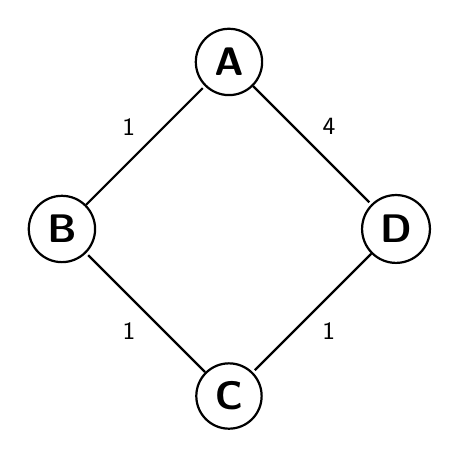
\begin{tikzpicture}[>=stealth',shorten >=1pt,auto,node distance=3cm,
  thick,main node/.style={circle,fill=white!20,draw,font=\sffamily\Large\bfseries}]

  \node[main node] (1) {A};
  \node[main node] (2) [below left of=1] {B};
  \node[main node] (3) [below right of=2] {C};
  \node[main node] (4) [below right of=1] {D};

  \path[every node/.style={font=\sffamily\small}]
    (1) edge node {4} (4)
    (2) edge node {1} (1)
    (3) edge node {1} (2)
    (4) edge node {1} (3);
\end{tikzpicture}
\caption{Graph with original weights}
\end{subfigure} \qquad
\begin{subfigure}[h]{0.3\textwidth}
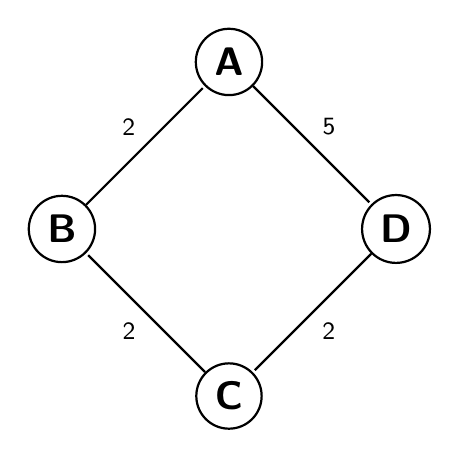
\begin{tikzpicture}[>=stealth',shorten >=1pt,auto,node distance=3cm,
  thick,main node/.style={circle,fill=white!20,draw,font=\sffamily\Large\bfseries}]

  \node[main node] (1) {A};
  \node[main node] (2) [below left of=1] {B};
  \node[main node] (3) [below right of=2] {C};
  \node[main node] (4) [below right of=1] {D};

  \path[every node/.style={font=\sffamily\small}]
    (1) edge node {5} (4)
    (2) edge node {2} (1)
    (3) edge node {2} (2)
    (4) edge node {2} (3);
\end{tikzpicture}
\caption{Graph with new weights}
\end{subfigure}
\end{figure}

\end{itemize}
\end{document}